\section{Introduction}
NEXT-DEMO is a high-pressure xenon TPC contained within a cylindrical stainless-steel pressure vessel of diameter 30~cm and length 60~cm which was designed to withstand up to 10~bar. The TPC itself is defined by three metallic wire grids --- called \emph{cathode}, \emph{gate} and \emph{anode} --- which define the two active regions: the 30-cm long \emph{drift region}, between cathode and gate with a  drift field up to 800~V~cm$^{-1}$; and the 5 mm long \emph{EL region}, between gate and anode.  The electric field is created by supplying a large negative voltage to the cathode, then degrading it using a series of metallic rings of 30 cm diameter spaced 5 mm and connected via 0.5~G$\Omega$ resistors (shown in figure~\ref{fig:TPC}).  The gate is at negative voltage so that a moderate electric field --- [1.0, 4.0]~$\mathrm{kV~cm^{-1}~bar^{-1}}$ --- is created between the gate and the anode, which is at ground. A set of six panels made of PTFE (Teflon) coated with tetraphenyl-butadiene (TPB) are mounted inside the electric-field cage forming a \emph{light tube} of hexagonal cross section with an apothem length of 8~cm. 


%%%%%%%%%%
\begin{figure}
\centering
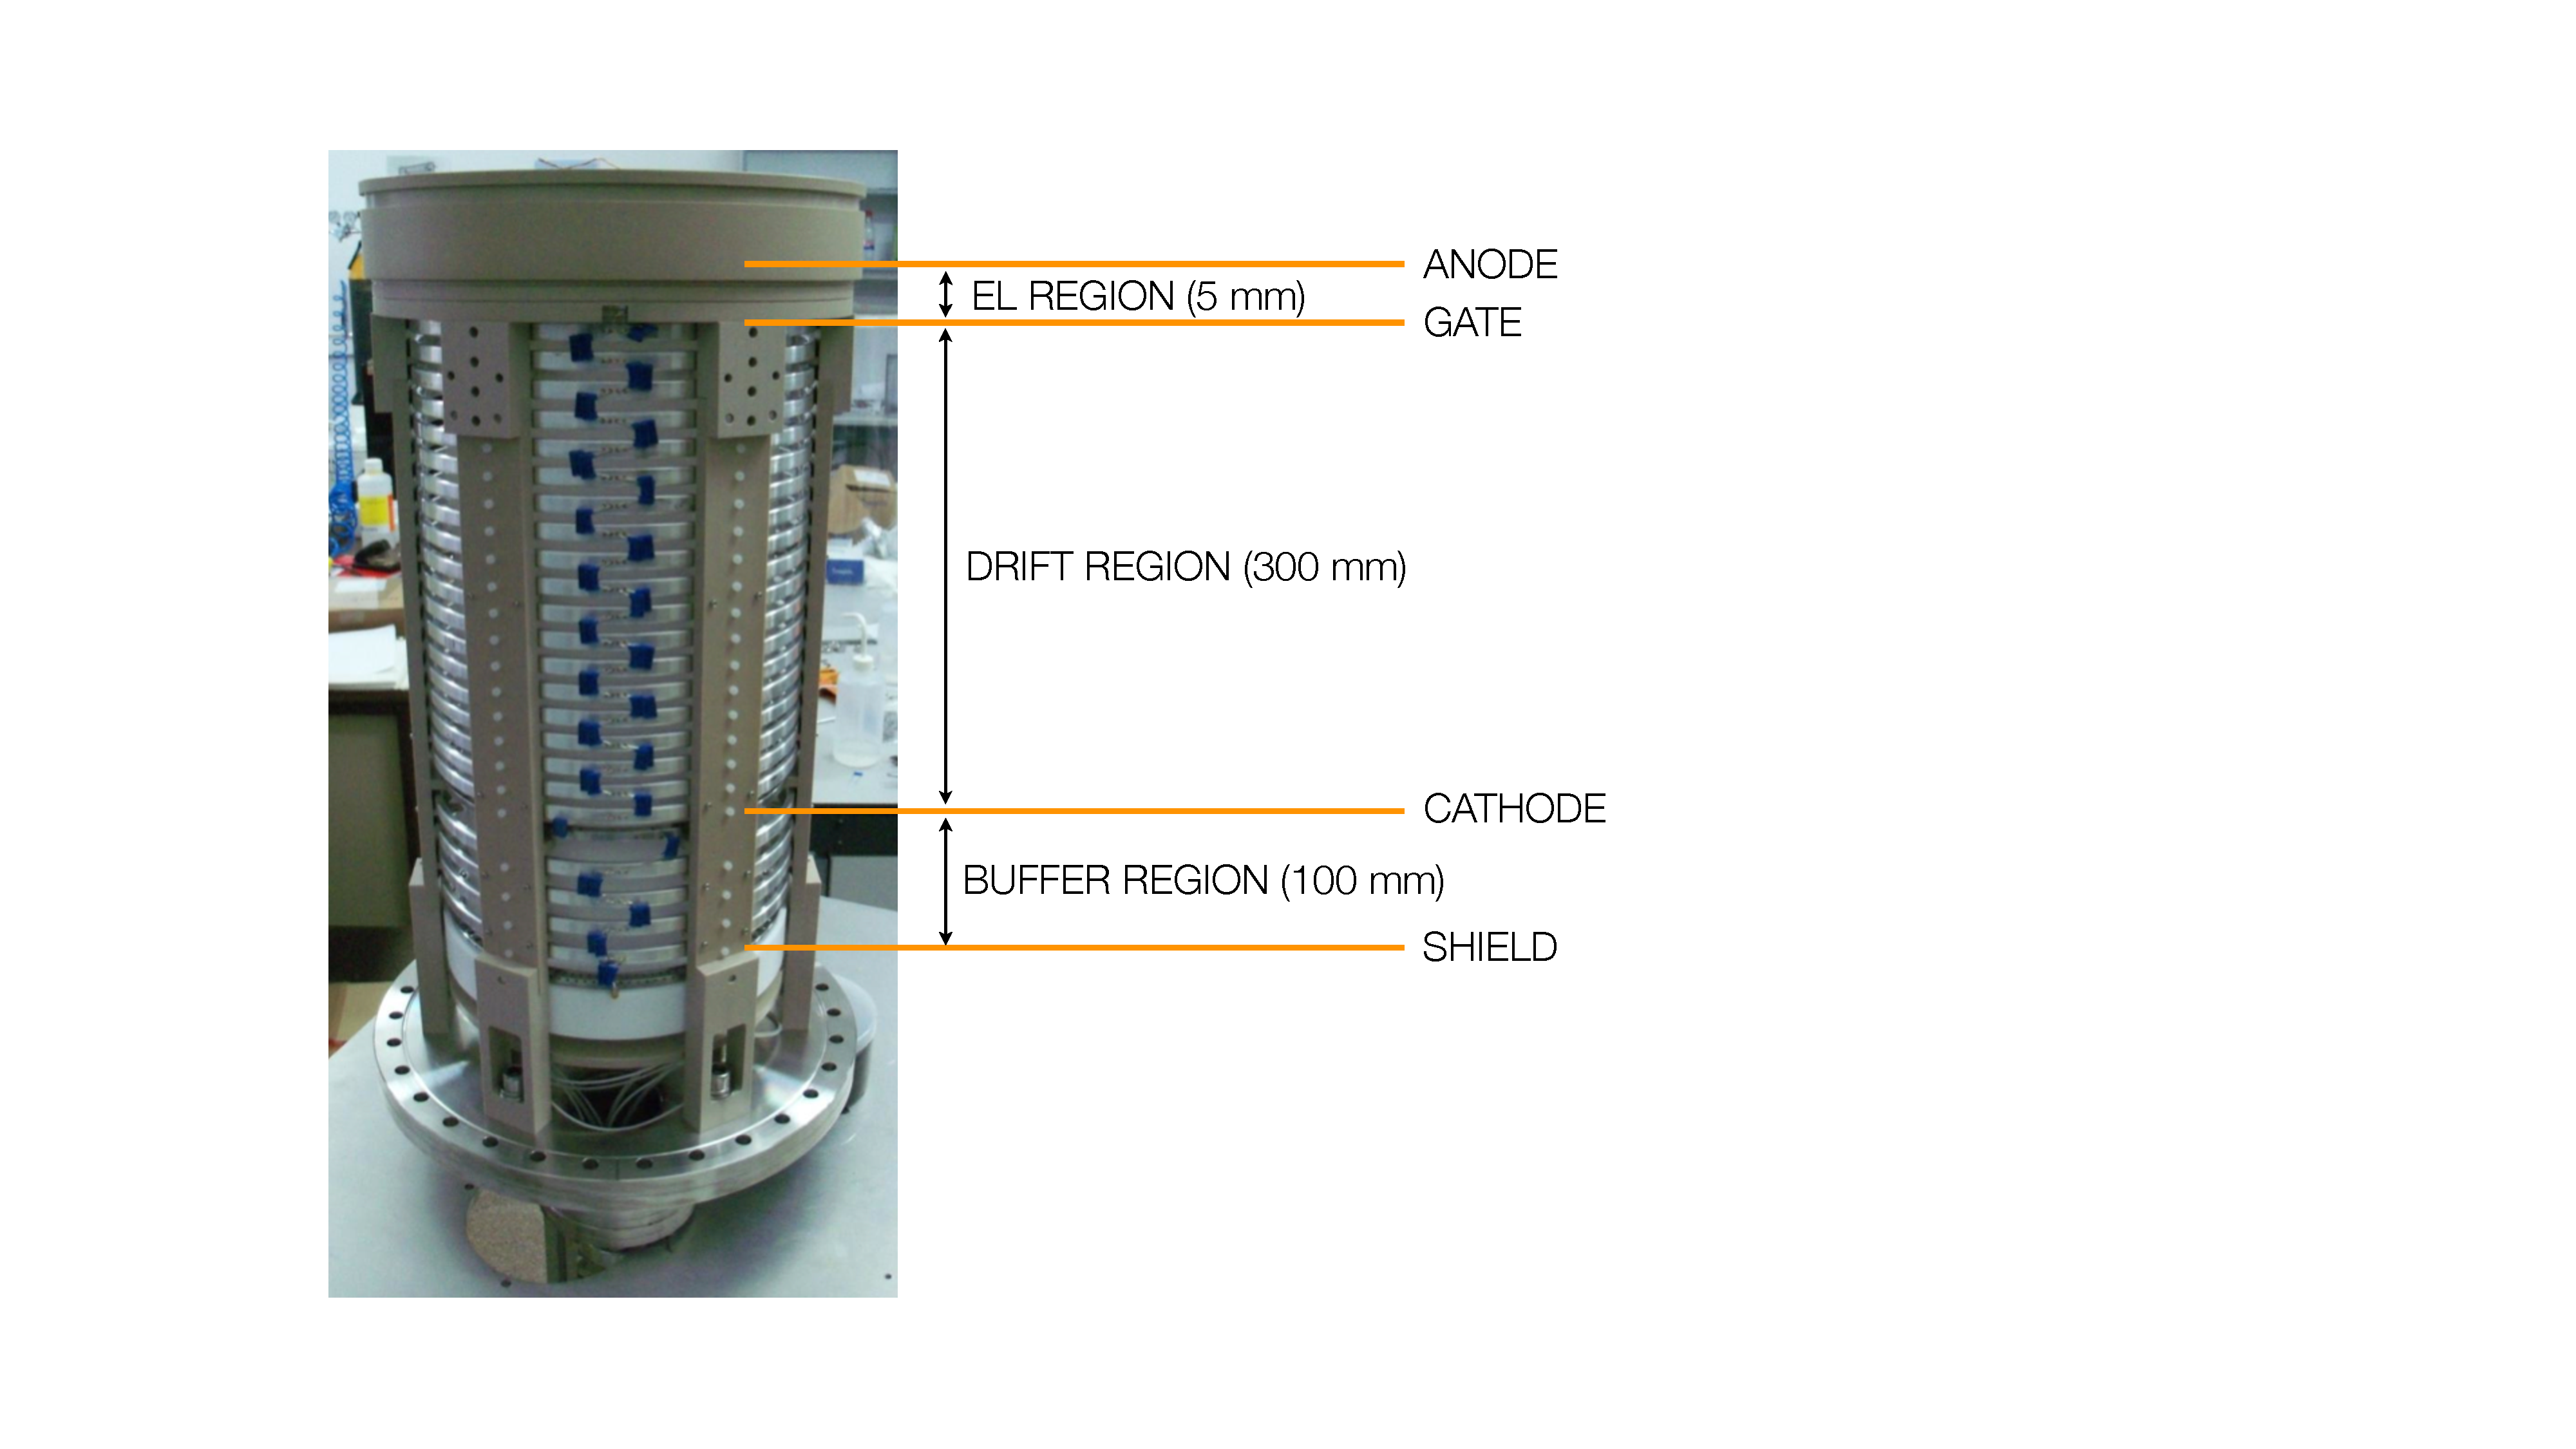
\includegraphics[width=0.75\textwidth]{img/FieldCage.pdf}
\caption{External view of the time projection chamber mounted on one end-cap. The approximate positions of the different regions of the TPC are indicated.} \label{fig:TPC}
\end{figure}
%%%%%%%%%%


The NEXT-DEMO detector has been operating continuously at IFIC (Figure \ref{fig:cleanroom} shows the NEXT-DEMO detector in the experimental are at IFIC )without major problems during the last three years (2011-2014). Its operation and results has been useful to fully demonstrate the capabilities of the NEXT technology for the search of the neutrinoless double beta decay process.


%%%%%%%%%%
\begin{figure}
\centering
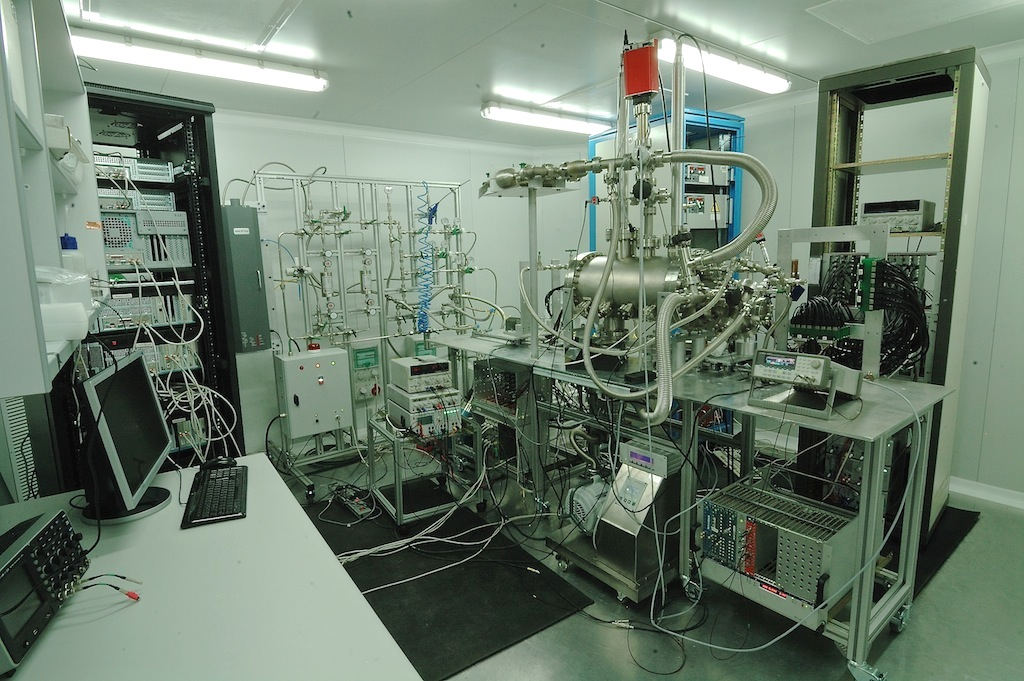
\includegraphics[width=0.75\textwidth]{img/NextDemo_cleanroom.jpg}
\caption{Picture of the NEXT-DEMO detector in the experimental area at IFIC with all the different systems needed for its operation: Gas system, High voltage modules and electronics.} \label{fig:cleanroom}
\end{figure}
%%%%%%%%%%

The next step for the NEXT-DEMO detector is to keep helping as a demonstrator for new ideas that can be implemented in larger detectors. In that sense, the possibility to use a magnetic field in parallel to the drift field of the TPC could give us an improvement in the background rejection factor of almost an order of magnitude with no significant lose of efficiency. This afirmation comes from our recent Monte-Carlo studies and it needs to be tested experimentally with a realistic set-up. Here the NEXT-DEMO detector seems to be the clear candidate.

The project that we propose to CERN consists in placing the NEXT-DEMO detector inside the HARP magnet at CERN and operate it in order to confirm the Monte-Carlo results.
